\documentclass{../templates/topic}

\begin{document}
\graphicspath{{assets/}{ch3a_Time_Domain_Performance_Characteristics/assets/}}

\chapter{The Complex Plane}

\begin{section}{Defintion}
	The complex plain is the plane formed by the Real and Complex number lines.
	
	It is useful when the roots and poles of a Transfer Function are plotted on it. It becomes a graphical tool which allows us to estimate the performance of a system.
	\subsection{Reading Parameters}
		The $(x,y)$ coordinates of a root correspond to the values $(\sigma, \omega_d)$ for that root.
		
		The distance of the root to the origin correspons to $\omega_n$ for that root.
		
		With the angle formed between the negative real number line and the root defined as $\alpha$, $\cos{\alpha}=\zeta$.
\end{section}

\begin{section}{Expressing Requirements on the Plane}
	
	Simple requirements can be expressed as follows:
	
	\begin{figure}
		\centering
		
		\begin{subfigure}[b]{0.4\textwidth}
		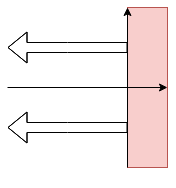
\includegraphics[width=\textwidth]{complex_plane_convergence.png}
		\caption{Quicker Convergence}
		\end{subfigure}
		% This line necessary
		\begin{subfigure}[b]{0.4\textwidth}
		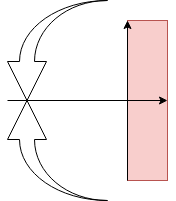
\includegraphics[width=\textwidth]{complex_plane_overshoot.png}
		\caption{Less Overshoot}
		\end{subfigure}
		\\
		\begin{subfigure}[b]{0.4\textwidth}
		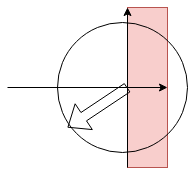
\includegraphics[width=\textwidth]{complex_plane_rise.png}
		\caption{Shorter Rise (radial)}
		\end{subfigure}
		% This line necessary
		\begin{subfigure}[b]{0.4\textwidth}
		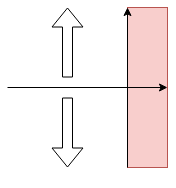
\includegraphics[width=\textwidth]{complex_plane_peak.png}
		\caption{Shorter Peak}
		\end{subfigure}

	\end{figure}
	
	Simply identify the value which makes the the condition true, and then block off the area below it on the graph.
	
	Composite requirements can be made by superimposing simple requirements.

\end{section}

\end{document}